%%This is a very basic article template.
%%There is just one section and two subsections.
\documentclass[a4paper]{article}

\usepackage{a4wide}
\usepackage{amsmath}
\usepackage{ltxtable}
\usepackage{graphicx}
\usepackage{float}
\usepackage{listings}

\begin{document}
\title{Numerical Optimization\\Project 2}
\author{Charalampos Kaidos}

\maketitle

\section{Algorithms}
The Gradient Descent, the Conjugate Gradient and the Preconditioned Conjugate Gradient algorithms were implemented.

\subsection{Gradient Descent}
\begin{quote}
	gradient\_descent.py
\end{quote}
The Gradient Descent is the simplest algorithm to iterative approach a solution of the problem $Ax=b$. The algorithm starting from an initial position $x_0$, calculates the gradient $\bigtriangledown F(x)$ at that position and then updates $x$ using the formula:
$$
x_{k+1}=x_k + a_k\bigtriangledown F(x_k)
$$

In the formula above $a_k$ is learning rate, usually a value $0<a<1$ which controls how far the $x$ moves. Smaller values of $a$ mean that the algorithm will need more iterations to converge, while larger values means that the algorithm may overshot the target and zig-zag over it or even miss it completely. There are several algorithms to update $a$ at each iteration, we used the steepest descent:
$$
a_k = \frac{r_k^Tr_k}{r_k^TAr_k}
$$
where $r_k = b - Ax_k$ is the residual at step $k$.

\begin{lstlisting}
func gd(A, b, x0){
	x = x0
	residual = b - Ax
	for i in [1...max iterations]{
		a = residual.T * residual / residual.T * A * residual
		x = x + a * residual
		residual = residual - a * residual
	}
}
\end{lstlisting}

\subsection{Conjugate Gradient}
\begin{quote}
	conjugate\_gradient.py
\end{quote}
The Conjugate Gradient algorithm is similar to the Gradient Descent in the sense that it updates $x_k$ at each step using a learning rate and a function of $x_{k-1}$, but this one also exploits knowledge about the convex of the function to achieve much faster convergence to the solution. Like the Gradient Descent it involves only one matrix-vector multiplication per iteration thus it has about the same complexity per iteration.

\begin{lstlisting}
func cg(A, b,  x0){
	x = x0
	residual = b - Ax
	direction = residual
	for i in [1...max iterations]{
		a = residual.T * residual / direction.t * A * direction
		x = x + a * direction
		residual = residual - a * A * direction
		b = residual.T * residual / prev_residual.T * prev_residual
		direction = residual + b * direction
	}
}
\end{lstlisting}

\subsection{Preconditioned Conjugate Gradient}
\begin{quote}
	preconditioned\_conjugate\_gradient.py
\end{quote}
The Preconditioned Conjugate Gradient method is similar to the Conjugate Gradient method but it also uses a preconditioning matrix to make the problem much faster to converge. The idea is the preconditioner matrix $P$ changes the coordinates such as $x = Py$, we solve the easier problem  $P^TAPy=P^Tb$ and then find $x* = T^{-1}y*$. In this algorithm we have one extra matrix-vector multiplication per iteration compared to Conjugate Gradient but we hope we will require much iterations to solve the problem.

\begin{lstlisting}
func pcg(A, b, x0, P){
	x = x0
	M = PP.T
	residual = b - Ax
	mod_residual = inv(M)*residual
	direction = mod_residual
	for i in [1...max iterations]{
		a = residual.T*mod_residual / direction.T * A * direction
		x = x + a * direction
		residual = residual - a * A * direction
		mod_residual = inv(M) * residual
		b = mod_residual.T * residual / prev_mod_residual.T * prev_residual
		direction = mod_residual + b * direction
	}
}
\end{lstlisting}

\subsection{Implemenation details}
All 3 algorithms require a multiplication of A with a vector within the iteration which is a $O(n^2)$ operation. Since we know that A is a Toeplitz matrix we can exploit its characteristics and make this operation faster. More specifically, we transform A to a circulant matrix C and then use FFT and an element wise vector multiplication to calculate the product. This  brings the computational complexity down to the cost of the FFT which is $O(nlogn)$.

Using the FFT method the algorithms need to store extra data in memory to achieve this faster performance (as always with algorithms there is a memory-computations trade off).

The Gradient Descent method needs to store table A ($O(n^2)$), and vectors b ($O(n)$), x0 ($O(n)$) in addition to complex vector g ($O(n)$) ($g=FFT(C_{2n}[:0])$), vector of residuals ($O(n)$) and vector of the product A*residual ($O(n)$).

The Conjugate Gradient method needs the same as Gradient Descent in addition to vector p of direction ($O(n)$), as well as the vectors of residuals ($O(n)$) and direction ($O(n)$) of the previous iteration.

Finally the Preconditioned Conjugate Gradient needs the same as Conjugate Gradient in addition to the inverse matrix $M^{-1}$ of $M = PP^T$ ($O(n^2)$), vector z of the product of $M^{-1}$ with the residual ($O(n)$) and the vector z of the previous iteration ($O(n)$).

\section{Gradient Descent and Conjugate Gradient}
\begin{quote}
	problem2.py
\end{quote}
On this section we will compare the gradient descent algorithm we implemented above against the Conjugate Gradient algorithm.

We execute both algorithms for the matrix $T_n$ with $n=2^l, l \in [9,13]$. The execution continues for 1000 iterations or until the algorithm converges when $\frac{\|r_m\|_2}{\|r_0\|_2} < 10^{-7}$ where $r_m$ is the residual at iteration $m$; $r_m = b - Ax_{m}$. In the matrix bellow  and figures \ref{fig:logtimegdcg1000} and \ref{fig:logitgdcg1000} we observe the results:

\begin{center}
	\begin{tabular}{r | c | c | c | c }
		& \multicolumn{2}{c}{Gradient Descent} & \multicolumn{2}{c}{Conjugate Gradient}\\ \hline
		n & Iterations & Time (s) & Iterations & Time (s)\\ \hline
		512 & 1000 & 0.11427203300000022 & 372 & 0.04848144600000004\\ \hline
		1024 & 1000 & 0.1336267499999999 & 767 & 0.11581877299999999\\ \hline
		2048 & 1000 & 0.21103424999999998 & 1000 & 0.2193386460000002\\ \hline
		4096 & 1000 & 0.3909173479999999 & 1000 & 0.3936477730000001\\ \hline
		8192 & 1000 & 0.7784238909999992 & 1000 & 0.7993831770000002\\ \hline
	\end{tabular} 
\end{center}

\begin{figure}[H]
	\centering
	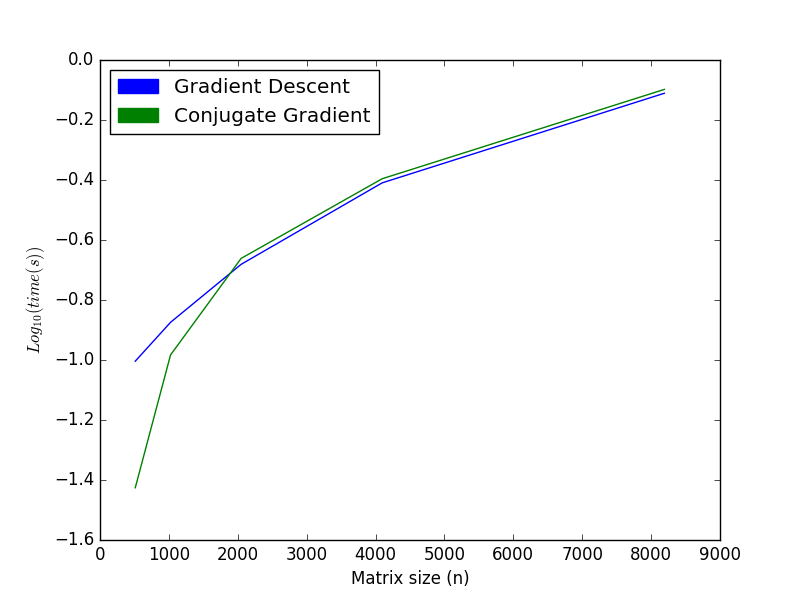
\includegraphics[width=1\textwidth]{2logtime1000.png}
	\caption{Log-Time for GD and CG}
	\label{fig:logtimegdcg1000}
\end{figure}

\begin{figure}[H]
	\centering
	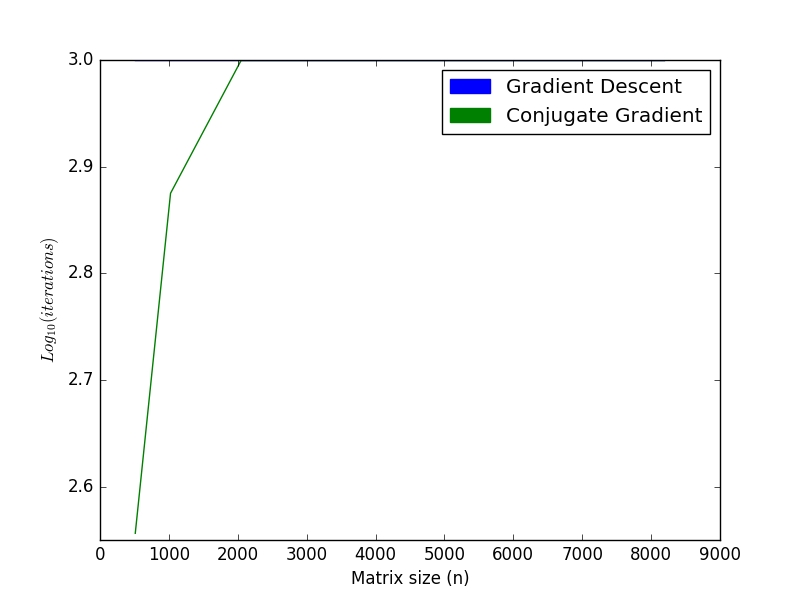
\includegraphics[width=1\textwidth]{2logiterations1000.png}
	\caption{Log-Iterations for GD and CG}
	\label{fig:logitgdcg1000}
\end{figure}

It appears as if both methods require the same amount of time, but this is not the case, it's just that both methods require about the same time per iteration and both stop at 1000 iterations.

It is obvious that 1000 iterations are not enough for Gradient Descent to converge, and Conjugate Gradient also doesn't converge for higher matrix sizes. If we increase the maximum number iterations to 1000000 we get the results as shown on table bellow and figures \ref{fig:logtimegdcg} and \ref{fig:logitgdcg}.

\begin{center}
	\begin{tabular}{r | c | c | c | c }
		& \multicolumn{2}{c}{Gradient Descent} & \multicolumn{2}{c}{Conjugate Gradient}\\ \hline
		n & Iterations & Time (s) & Iterations & Time (s)\\ \hline
		512 & 1000000 & 96.63653615 & 372 & 0.0394357430000003\\ \hline
		1024 & 1000000 & 131.583186959 & 767 & 0.10563208199999963\\ \hline
		2048 & 1000000 & 215.47961726300002 & 1562 & 0.33579735700001834\\ \hline
		4096 & 1000000 & 394.8912016549999 & 3161 & 1.2406785360000185\\ \hline
		8192 & 1000000 & 812.2607948849999 & 6367 & 5.162610887000028\\ \hline
	\end{tabular} 
\end{center}

\begin{figure}[H]
	\centering
	\includegraphics[width=1\textwidth]{2time.png}
	\caption{Time for GD and CG}
	\label{fig:timegdcg}
\end{figure}

\begin{figure}[H]
	\centering
	\includegraphics[width=1\textwidth]{2logtime.png}
	\caption{Log-Time for GD and CG}
	\label{fig:logtimegdcg}
\end{figure}

\begin{figure}[H]
	\centering
	\includegraphics[width=1\textwidth]{2iterations.png}
	\caption{Iterations for GD and CG}
	\label{fig:itgdcg}
\end{figure}

\begin{figure}[H]
	\centering
	\includegraphics[width=1\textwidth]{2logiterations.png}
	\caption{Log-Iterations for GD and CG}
	\label{fig:logitgdcg}
\end{figure}

Again the Gradient Descent didn't manage to converge (the algorithm converges for matrix size 512 at about 1500000 iterations and for 1024 at 18000000 iterations based on further tests) but the Conjugate Gradient did and there are interesting observations.

First of all each iteration in both algorithms has about the same cost; for $n=8192$ it is 0.0008s per iteration on this CPU ($\frac{812.26s}{1000000} \approx \frac{5.16s}{6367}$).

Also the increase in computational complexity is sub-exponential; there is a slight curve in the time graph of Gradient Descent in figures \ref{fig:timegdcg}  and \ref{fig:logtimegdcg} where the algorithm has executed 1000000 iteration on each matrix size. This is to be expected as it is dominated by the FFT which is $O(nlogn)$ complexity.

Next we observe from figure \ref{fig:logitgdcg} and the table above that Conjugate Gradient is linear to the amount of iterations required to converge as the matrix size increases which is expected; the CG method converges in at most n iterations (with infinite precision; here we have set a value of "good enough" convergence).

Finally the obvious, the conjugate gradient method requires much much less iterations than the gradient descent method to converge on the same problem.

From the iterations needed to converge we can calculate a lower bound for the condition number of each matrix:
\begin{align}
\|x - x_k\| &\le 2(\frac{\sqrt{c} - 1}{\sqrt{c} + 1})^k\|x - x_0\|\nonumber\\
\frac{\|x - x_k\|}{\|x - x_0\|} &\le 2(\frac{\sqrt{c} - 1}{\sqrt{c} + 1})^k\nonumber\\
10^{-7} &\le 2(\frac{\sqrt{c} - 1}{\sqrt{c} + 1})^k\nonumber\\
-7 &\le k\log_{10}(2\frac{\sqrt{c} - 1}{\sqrt{c} + 1})\nonumber\\
-\frac{7}{k} &\le \log_{10}(2\frac{\sqrt{c} - 1}{\sqrt{c} + 1})\nonumber\\
10^{-\frac{7}{k}} &\le 2\frac{\sqrt{c} - 1}{\sqrt{c} + 1}\nonumber\\
\sqrt{c}10^{-\frac{7}{k}} + 10^{-\frac{7}{k}} &\le 2\sqrt{c}-2\nonumber\\
\sqrt{c}(10^{-\frac{7}{k}}-2) &\le -2 - 10^{-\frac{7}{k}}\nonumber\\
\sqrt{c}(2 - 10^{-\frac{7}{k}}) &\ge 2 + 10^{-\frac{7}{k}}\nonumber\\
\sqrt{c} &\ge \frac{2 + 10^{-\frac{7}{k}}}{2 - 10^{-\frac{7}{k}}}\nonumber\\
c &\ge (\frac{2 + 10^{-\frac{7}{k}}}{2 - 10^{-\frac{7}{k}}})^2\nonumber\\
\end{align}

Solving for each number of iterations observed we get the following table where the condition number increases logarithmically:
\begin{center}
	\begin{tabular}{r | c | c}
		n & Iterations & Condition number $\ge$\\ \hline
		512 & 372 & 8.050201216864723\\ \hline
		1024 & 767 & 8.517722331333921\\ \hline
		2048 & 1562 & 8.757775861958155\\ \hline
		4096 & 3161 & 8.878961689710614\\ \hline
		8192 & 6367 & 8.939575495604588\\ \hline
	\end{tabular} 
\end{center}

\section{Preconditioned Conjugate Gradient}
\begin{quote}
	problem3.py
\end{quote}
On this section we executed the Preconditioned Conjugate Gradient algorithm on the same data using the tridiagonal matrix $[-1 2 -1]$ as preconditioner. We expect this algorithm to achieve faster convergence than the Conjugate Gradient as the preconditioning will stabilize the condition of the matrix A as n increases. We executed the algorithm for matrixes of size 64 to 8192 in order to compare with the previous execution:

\begin{center}
	\begin{tabular}{r | c | c}
		n & Iterations & Time (s)\\ \hline
		64 & 34 & 0.0035231849999999287\\ \hline
		128 & 68 & 0.010128990999999976\\ \hline
		256 & 145 & 0.049424055999999994\\ \hline
		512 & 307 & 0.318908894\\ \hline
		1024 & 679 & 2.820886541\\ \hline
		2048 & 1544 & 22.721836424\\ \hline
		4096 & 3629 & 186.36075025\\ \hline
		8192 & 8526 & 1555.297202325\\ \hline
	\end{tabular} 
\end{center}

\begin{figure}[H]
	\centering
	\includegraphics[width=1\textwidth]{3time.png}
	\caption{Time for PCG}
	\label{fig:3timegdcg}
\end{figure}

\begin{figure}[H]
	\centering
	\includegraphics[width=1\textwidth]{3logtime.png}
	\caption{Log-Time for PCG}
	\label{fig:3logtimegdcg}
\end{figure}

\begin{figure}[H]
	\centering
	\includegraphics[width=1\textwidth]{3iterations.png}
	\caption{Iterations for PCG}
	\label{fig:3itgdcg}
\end{figure}

\begin{figure}[H]
	\centering
	\includegraphics[width=1\textwidth]{3logiterations.png}
	\caption{Log-Iterations for PCG}
	\label{fig:3logitgdcg}
\end{figure}

We observe that the algorithm initially requires less iterations that the CG but this advantage fades away as the matrix size increases. Also the execution time is much slower as each iteration needs to perform one extra matrix multiplication that cannot be sped up with FFT ($M{-1}$) is not Toeplitz or Circulant and also a matrix inversion is needed during setup which is an ($O(n^3)$) operation and can add significant computation.

\section{Matrix Contidion}
\begin{quote}
	problem4.py
\end{quote}
We calculated the eigenvalues of matrices $T_n$ and $P^{-1}T_n$ for different values of n and we can see the results in figures \ref{fig:4condition} and \ref{fig:4logcondition}.

\begin{figure}[H]
	\centering
	\includegraphics[width=1\textwidth]{4condition.png}
	\caption{Condition}
	\label{fig:4condition}
\end{figure}

\begin{figure}[H]
	\centering
	\includegraphics[width=1\textwidth]{4logcondition.png}
	\caption{Log-Condition}
	\label{fig:4logcondition}
\end{figure}

While the condition number of $T_{-1}$ seems to be growing with rate close to $nlogn$ the condition number of $P^{-1}T_n$ is practically constant at 2.5.

\section{Cholesky direct method}
\begin{quote}
	problem5.py
\end{quote}
The Cholesky method attempts to break a large problem A into to smaller ones $L$ and $L^T$ which are triangular matrices. It is a direct method. We used numpy's implementation of Cholesky decomposition and the accompanying solver for a problem of size $2^{13}$. The results and comparison to PCG:

\begin{center}
	\begin{tabular}{r | c }
		Method & Time (s)\\ \hline
		Cholesky & 24.199078143999998s\\ \hline
		PCG & 1555.297202325\\ \hline
		CG & 5.162610887000028\\ \hline
	\end{tabular} 
\end{center}

It is obvious that the direct method of Cholesky is much faster than PCG in this problem, but CG remains the fastest of the 3. Actually the Cholesky method is 98\% faster the PCG and the CG method is 80\% faster than PCG.


\end{document}
